\chapter{Anwendung von LLM Tools im Software Engineering} \index{Anwendung von LLM Tools im Software Engineering}

Dieses Kapitel befasst sich mit der Frage, wie LLM Tools im Software Engineering Prozess unterstützen können.
Grundsätzlich gibt es da natürlich zahlreiche Möglichkeiten, die unmöglich alle im Rahmen einer Arbeit untersucht 
werden können. Daher widmet sich die Arbeit eher der selbstständigen Erstellung der Dokumente als der Unterstützung bei 
der Pflege oder ähnlichen Unterstützungsmöglichkeiten. Dazu wird im folgenden zu jedem Dokument beschrieben,
was im anschließenden Kapitel ``Praxisergebnisse und Vergleich'' betrachtet wird. Die \autoref{Dokumente mit LLM}
zeigt eine Tabelle mit möglichen KI Unterstützungen im Bezug auf die Inhalte der einzelnen Dokumente und soll einen kurzen 
Überblick dazu abbilden.

\begin{figure}[H]
    \centering
    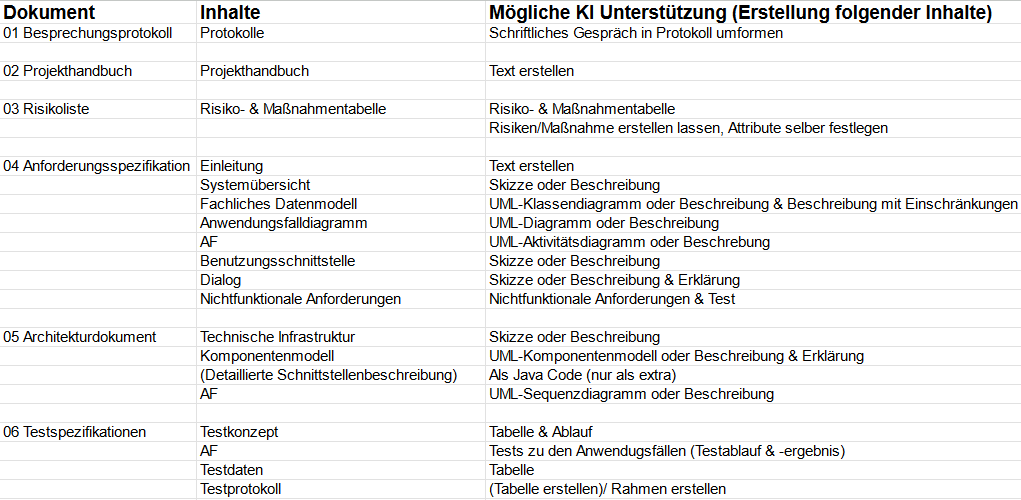
\includegraphics[width=\textwidth]{pictures/TabelleKap3.PNG}
    \caption{Mögliche LLM Tool Unterstützung}
    \label{Dokumente mit LLM}
\end{figure}

\section{Besprechungsprotokoll} \index{Besprechungsprotokoll} \label{LLMBesprechungsprotokoll}

Im \autoref{Besprechungsprotokoll} wurde bereits erläutert, welche Inhalte in einem Besprechungsprotokoll enthalten 
sind. Nun stellt sich die Frage, wie LLM-Tools bei der Erstellung eines solchen Dokuments unterstützen können.

Eine Möglichkeit wäre, das Besprechungsprotokoll aufzeichnen zu lassen und anschließend automatisch daraus das 
Protokoll zu erstellen. Dies wird jedoch in dieser Arbeit nicht betrachtet, da lediglich bei der kostenfreien Version 
ChatGPT-4o Dokumente als Eingabe genutzt werden können. Daher wäre dies nur in einem begrenzten Umfang und ohne Vergleiche 
testbar.

Eine alternative Möglichkeit wäre, das Meeting zu verschriftlichen und die schriftlichen Inhalte als Texteingabe zu 
verwenden. Mithilfe dieses schriftlichen Gesprächs könnten die Tools dann automatisch die Tabelle des 
Besprechungsprotokolls erstellen. Die zu Beginn des Besprechungsprotokolls aufgelisteten Daten – Datum, Thema, 
Verfasser, Teilnehmer und Verteiler – könnten dabei vernachlässigt werden, da diese Informationen vermutlich separat 
in die Eingabe eingefügt werden müssten, um erstellt zu werden. Dadurch gäbe es keine Zeitersparnis oder sonstigen 
Vorteil, sich diese Informationen automatisch erstellen zu lassen.


\section{Projekthandbuch} \index{Projekthandbuch} \label{LLMProjekthandbuch}

Das Projekthandbuch ist ein zentrales Dokument im Software Engineering Prozess, das alle wesentlichen Informationen und 
Richtlinien eines Projekts zusammenfasst. Die spezifischen Inhalte dieses Dokuments wurden bereits im 
\autoref{Projekthandbuch} dargelegt. Doch wie können LLM-Tools bei der Erstellung des 
Projekthandbuches unterstützend wirken?

Im Rahmen dieser Arbeit wird sich auf die Abschnitte ``Zweck des Dokuments'', ``Redaktion'' und ``Verteiler'' im Kapitel 
``Einleitung'' des Projekthandbuches sowie auf die Abschnitte ``Vorgeschichte'' und ``Inhaltliche Kurzdarstellung'' im 
Kapitel ``Projektdefinition'' beschränkt. Der Grund dafür ist, dass die restlichen Abschnitte des Projekthandbuchs aus den 
Unterlagen für das Modul ``Secure Software Engineering'' stammen und hauptsächlich als Bild aus der Präsentation in das 
Projekthandbuch eingefügt werden.\\
Die aufgezählten Abschnitte könnten automatisch erstellt werden. Falls spezifische Informationen dafür benötigt 
werden, müssten diese in die Eingabe integriert werden.

\section{Risikoliste} \index{Risikoliste} \label{LLMRisikoliste}

Nachdem im \autoref{Risikoliste} die Bestandteile der Risikoliste beschrieben wurden, stellt sich auch hier die Frage, 
wie LLM Tools bei der Erstellung und Pflege der Risikoliste mitwirken und unterstützen können.

Eine Möglichkeit besteht darin, die gesamte Risikoliste einschließlich der zugehörigen Maßnahmentabelle von LLM Tools 
erstellen zu lassen. Dabei sollten alle Attribute für die Risiken klar festgelegt werden. Zudem sollten die Werte 
der einzelnen Risikoattribute in einem konsistenten Verhältnis zueinander stehen.


\section{Anforderungsspezifikation} \index{Anforderungsspezifikation} \label{LLMAnforderungsspezifikation}

Der \autoref{Anforderungsspezifikation} beschreibt die einzelnen Inhalte der Anforderungsspezifikation. Doch wie 
können LLM-Tools bei der Erstellung dieser unterstützen?

Zunächst könnte die Einleitung des Dokuments vollständig von den Tools erstellt werden. Falls hierfür spezifische 
Informationen benötigt werden, sollten diese in die Eingabe integriert werden.

Anschließend folgt die Systemübersicht. Da außer ChatGPT-4o keines der Tools eigenständig Dokumente erstellen kann, 
wird die Zeichnung vermutlich selbst erstellt werden müssen. Es sollte jedoch möglich sein, die Beschreibung der 
Komponenten und deren Beziehungen von den Tools erstellen zu lassen und diese dann in eine Zeichnung umzusetzen. 
Ebenso kann der Text, der das System beschreibt und in die Systemlandschaft einordnet, automatisch generiert werden. 
Der Fokus liegt hier jedoch auf der Zeichnung sowie auf der Beschreibung der Komponenten und deren Beziehungen.

Ähnlich verhält es sich beim fachlichen Datenmodell. Hier könnte das UML-Klassendiagramm als PlantUML-Code oder 
in einem ähnlichen Format ausgegeben werden. Da dies jedoch eher an den Programmierfähigkeiten scheitert als an 
der Fähigkeit, ein fachliches Datenmodell zu erstellen, fließt es nicht negativ in die Bewertung ein, wenn dieses 
nicht erstellt werden kann. Die Beschreibung des Diagramms sollte allerdings so präzise sein, dass die Erstellung 
des Diagramms manuell erfolgen kann. Die dazugehörigen Beschreibungen und Einschränkungen können ebenfalls von den 
Tools generiert werden.

Anschließend folgt das Anwendungsfalldiagramm. Dieses könnte ebenfalls mittels PlantUML oder ähnlichen Tools 
grafisch erstellt werden, was jedoch aus den oben genannten Gründen keine Voraussetzung ist. Alternativ können 
die LLM-Tools die Rollen, deren Verbindungen und die zugehörigen Anwendungsfälle auflisten. Falls zusätzliche 
Bemerkungen zu den Anwendungsfällen erforderlich sind, können diese ebenfalls von den Tools erstellt werden.

Bei den detaillierten Beschreibungen der einzelnen Anwendungsfälle mit Aktivitätsdiagramm sollte der Fokus auf 
dem Aktivitätsdiagramm und den dazugehörigen Beschreibungen der Aktivitäten liegen. Das Aktivitätsdiagramm 
könnte ebenfalls mit PlantUML oder ähnlichen Tools erstellt werden. Dies ist aber auch hier keine Anforderung an 
die Tools, aufgrund den oben angegebenen Gründen. Falls dies jedoch nicht erstellt werden kann, ist eine genaue 
und detaillierte Beschreibung des Aktivitätsdiagramms erforderlich. Die Beschreibung der Aktivitäten 
sollte, unabhängig von der Darstellung des Diagramms, vollständig von den Tools generiert werden können.

Darauf folgt die Benutzungsschnittstelle, welche entweder vollständig durch PlantUML-Code oder ähnlichen Tools 
oder textuell beschrieben werden sollte. Die zusätzlichen Bemerkungen und die Zuordnung der Dialoge zu den Anwendungsfällen 
spielen hier erst einmal eine untergeordnete Rolle.

Die einzelnen Dialoge können textuell beschrieben oder im Chat skizziert werden, wobei es den Tools überlassen 
bleibt, welche Methode sie wählen. Die einzelnen Eingabefelder und Buttons sollten dabei erläutert werden. 
Die Beschreibung, wann der Dialog aufgerufen wird und was beim Schließen des Dialogs passiert, spielt zunächst 
eine untergeordnete Rolle.

Zuletzt werden die nichtfunktionalen Anforderungen mitsamt den dazugehörigen Tests aufgelistet. Beides sollte 
von den Tools eigenständig erstellt werden können.

\section{Architekturdokument} \index{Architekturdokument} \label{LLMArchitekturdokument}

Das Architekturdokument beschreibt die grundlegende Struktur und die Designentscheidungen eines Softwareprojekts. 
Die genauen Inhalte wurden bereits im \autoref{Architekturdokument} erläutert. In welchem Maße bestehen hier 
Unterstützungsmöglichkeiten durch LLM-Tools?

Die technische Infrastruktur besteht aus einer Grafik und einem erläuternden Text. Die Grafik kann optional als 
``Skizze'' im Chat erstellt werden, was jedoch keine zwingende Anforderung an die verwendeten Tools darstellt. 
Wenn eine Skizze erstellt wird, sollte auch ein erläuternder Text hinzugefügt werden. Andernfalls liegt der 
Fokus auf der textuellen Ausarbeitung. Dabei ist es zunächst unerheblich, ob der Text in Stichpunkten oder als 
Fließtext verfasst wird.

Anschließend folgt das Komponentenmodell, das optional wieder in PlantUML oder ähnlichen Tools erstellt werden 
kann. Alternativ kann auch eine detaillierte Beschreibung angefertigt werden. Dazu gehört ein begleitender Text, 
der die Komponenten und Schnittstellen beschreibt und deren Funktion erläutert. Ob dieser Text in Stichpunkten 
oder als Fließtext verfasst wird, spielt auch hier keine Rolle. Das Hauptaugenmerk liegt auf dem Komponentenmodell.

Nach der Schnittstellenbeschreibung folgt die dynamische Beschreibung exemplarischer Anwendungsfälle. Diese umfasst 
ein Sequenzdiagramm sowie die für den Anwendungsfall erforderlichen Vorbedingungen. Das Sequenzdiagramm kann ebenfalls 
als PlantUML-Code oder mit ähnlichen Tools erstellt werden, was jedoch keine zwingende Anforderung darstellt. Sollte 
dies nicht möglich sein, genügt auch eine detaillierte Beschreibung des Diagramms. Die Vorbedingungen sollten ohne 
größere Schwierigkeiten erstellt werden können, wobei sie hier zunächst von untergeordneter Bedeutung sind. Das 
Hauptaugenmerk liegt erneut auf dem Diagramm.

\section{Testspezifikation} \index{Testspezifikation} \label{LLMTestspezifikation}

Im \autoref{Testspezifikation} wurde bereits erklärt, welche Inhalte die Testspezifikation umfasst. Wie wäre hier eine 
Unterstützung durch LLM-Tools möglich?

Zunächst wird das Testkonzept betrachtet. Dieses kann automatisch generiert werden. Falls das generierte Konzept nicht den 
eigenen Vorstellungen entspricht, kann man zunächst Stichpunkte selbst schreiben und sich dann den Text daraus 
erstellen lassen. Auch die dazugehörige Tabelle sollte sich von den LLM-Tools erstellen lassen.

Anschließend folgen die Tests für die einzelnen Anwendungsfälle. Die Testfälle kann man vollständig von den Tools 
erstellen lassen. Die Testdaten, die bei diesen Tests benötigt werden, werden in einer Tabelle zusammengefasst. 
Auch diese Tabelle könnten die Tools automatisch generieren.

Die unausgefüllte Tabelle des Testprotokolls, z.B. Spalten- und Zeilenbeschriftung, könnte ebenfalls von den LLM-Tools erstellt werden. Die Ergebnisse 
könnten die Tools auch in die Tabelle mit eintragen, diese müssten allerdings in der Eingabe mit gegeben werden. 
Allerdings stellt sich hier in beiden Fällen die Frage, ob dies zu einer Zeitersparnis oder einer Arbeitserleichterung führt.